\chapter{Toepassingen van diepte-eerst zoeken}
\section{Enkelvoudige samenhang van grafen}
\subsection{Samenhangende componenten van een ongerichte graaf}
\begin{itemize}
	\item Een \textbf{samenhangende ongerichte graaf} is een graaf waarbij er een weg bestaat tussen elk paar knopen.
	\item Een \textbf{niet samenhangende ongerichte graaf} bestaat dan uit zo groot mogelijke samenhangende componenten.
\end{itemize}

\subsection{Sterk samenhangende componenten van een gerichte graaf}
\begin{itemize}
	\item Een \textbf{sterk samenhangende gerichte graaf} is een graaf waarbij er een weg tussen elk paar knopen in beide richtingen (niet perse dezelfde verbindingen) bestaat (cfr. figuur \ref{fig:sterk_samenhangende_graaf}).
	\begin{figure}[ht]
		\centering
		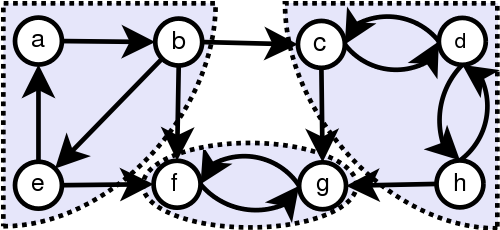
\includegraphics[width=0.5\textwidth]{img/sterk_samenhangende_graaf}
		\caption{Een sterk samenhangende graaf.}
		\label{fig:sterk_samenhangende_graaf}
	\end{figure}
				
	\item Een \textbf{zwak samenhangende gerichte graaf} is een graaf die niet sterk, maar toch samenhangend is indien de richtingen buiten beschouwing gelaten worden. Een graaf die niet sterk samenhangend is, bestaat uit zo groot mogelijke sterk samenhangende componenten. 
	\item Sommige algoritmen gaan ervan uit de een graaf sterk samenhangend is. Men moet dus eerst deze componenten bepalen, meestal via een \textbf{componentengraaf} die:
	\begin{itemize}
		\item een knoop heeft voor elk sterk samenhangend component,
		\item en een verbinding van knoop $a$ naar knoop $b$ indien er in de originele graaf een verbinding van één van de knopen van $a$ naar één van de knopen van $b$ is. 
	\end{itemize}
	\item De componentgraaf bevat geen lussen, anders wil dit zeggen dat die knoop zelf nog opgesplitst zou kunnen worden in twee sterk samenhangende componenten.
	\item De sterk samenhangende componenten kunnen bekomen worden met behulp van diepte-eerst zoeken (Kosaraju's Algorithm):
	\begin{enumerate}
		\item Stel de omgekeerde graaf op, door de richting van elke verbinding om te keren.
		\item Pas diepte-eerst zoeken toe op deze omgekeerde graaf, waarbij de knopen in postorder genummered worden.
		\item Pas diepte-eerst zoeken toe op de originele graaf, met als startknoop de resterende knoop met het hoogste postordernummer. Het resultaat is een diepte-eerst bos, waarvan de bomen sterk samenhangende componenten zijn.
	\end{enumerate}
	\item Diepte-eerst zoeken is $\Theta(n + m)$ voor ijle en $\Theta(n^2)$ voor dichte grafen. Het omkeren van de graaf is ook $\Theta(n + m)$ voor ijle en $\Theta(n^2)$ voor dichte grafen.
\end{itemize}




\section{Dubbele samenhang van ongerichte grafen}
Twee definities:
\begin{itemize}
	\item \textbf{Brug.} Een brug is een verbinding dat, indien deze wordt weggenomen, de graaf in twee deelgrafen opsplitst. Een graaf zonder bruggen noemt men \underline{dubbel lijnsamenhangend}; als er tussen elk paar knopen minstens twee onafhankelijke wegen bestaan, dan is een graaf zeker dubbel lijnsamenhangend.
	\item \textbf{Scharnierpunt.} Een scharnierpunt is een knoop dat, indien deze wordt weggenomen, de graaf in ten minste twee deelgrafen opsplitst. Een graaf zonder scharnierpunten noemt men \underline{dubbel knoopsamenhangend} (of dubbel samenhangend). Een graaf met scharnierpunten kan onderverdeeld worden in dubbel knoopsamenhangende componenten. Als er tussen elk paar knopen twee onafhankelijke wegen bestaan, dan is de graaf dubbel knoopsamenhangend.
\end{itemize}

Scharnierpunten, dubbel knoopsamenhangende componenten, bruggen en dubbel lijnsamenhangende componenten kunnen opnieuw via diepte-eerst zoeken gevonden worden:
\begin{enumerate}
	\item Stel de diepte-eerst boom op, waarbij de knopen in postorder genummerd worden. 
	\item Bepaal voor elke knoop $u$ de laagst genummerde knoop die vanuit $u$ kan bereikt worden via een weg bestaande uit nul of meer dalende boomtakken gevolgd door één terugverbinding. 
	\item Indien alle kinderen van een knoop op die manier een knoop kunnen bereiken die hoger in de boom ligt dan hemzelf, dan is de knoop zeker niet samenhangend. De wortel is een scharnierpunt indien hij meer dan één kind in heeft. \todo{hoe bruggen vinden?}
\end{enumerate}
Diepte-eerst zoeken is $\Theta(n + m)$ voor ijle en $\Theta(n^2)$ voor dichte grafen.
\section{Eulergraaf}
Een eulercircuit is een gesloten omloop in een graaf die alle verbindingen éénmaal bevat. Een eulergraaf is een graaf met een eulercircuit, die volgende eigenschappen heeft:
\begin{itemize}
	\item De graaf is knoopsamenhangend.
	\item De graad van elke knoop is even.
	\item De verbindingen kunnen onderverdeeld worden in lussen, waarbij elke verbinding slechts behoort tot één enkel lus.
\end{itemize}